% XeLaTeX document
\documentclass[12pt,a4paper]{article}

% Редактируем: конфигурация, личные настройки: имя, название предмета и пр. для титульной страницы и метаданных документа здесь
\include{config}

% Не редактируем: используемые пакеты
\include{settings/packages}

% Не редактируем: параметры используемых пакетов и не только
\include{settings/preferences}

% водяной знак для обозначения статуса документа

\begin{document}
% Не редактируем: Титульная страница (формируется автоматически из заданной конфигурации)
\include{templates/titlepage}

% Не редактируем: Страница содержания (формируется автоматически из section, subsection и пр., указанных в content.tex)
\include{templates/tocpage}

\listoffigures

% Редактируем: всё остальное: вступление, др. этапы, заключение, приложение
\section{Постановка задачи}
Необходимо сгенерировать массивы данных для пяти распределений:
\begin{itemize}
\item нормальное распределение \( N(x, 0, 1) \)
\item распределение Коши \( C(x, 0, 1) \)
\item распределение Лапласа \( L(x, 0, 1/\sqrt{2}) \)
\item распределение Пуассона \( P(k, 10) \)
\item равномерное распределение \( U(x, -\sqrt{3}, \sqrt{3}) \)
\end{itemize}
Для каждого распределения массивы должны состоять из 20 и 100 элементов. Для выборок построить боксплот Тьюки. Для каждого распределения определить долю выбросов экспериментально, сгенерировав выборку, соответствующую распределению 1000 раз, и вычислив среднюю долю выбросов, и сравнить с результатами, полученными теоретически.


\section{Теория}
Границами ящика служат первый и третий квартили, линия в середине ящика — медиана. Концы усов — края статистически значимой выборки и в нашем случае они равны разности первого квартиля и полутора межквартильных расстояний и сумме третьего квартиля и полутора межквартильных расстояний. Приведём формулы:
\[X_1 = Q_1 - k(Q_3 - Q_1)\] \[X_2 = Q_3 + k(Q_3 - Q_1)\] \[k = \frac{3}{2}\]
Здесь \(Q_1\) и \(Q_3\) - первый и третий квартили соответственно.
Выбросы отмечаются на графике в виде отдельных выколотых точек.
\\
\\
С помощью функций распределения можно вычислить теоретические значения нижнего и верхнего квартилей и по ним вычислить \(X_1^{T}\) и \(X_2^{T}\). После этого можно вычислить теоретическую долю выбросов:
\[P_в^{T} = P(x < X_1^{T}) + P(x > X_2^{T}) \]



\section{Реализация}
\begin{itemize}
\item Язык: Python
\item Среда разработки: PyCharm
\item Используемые библиотеки: NumPy, SciPy, MatPlotLib
\end{itemize}


\section{Результаты}

\subsection{Нормальное распределение}
\begin{figure}[H]
	\begin{center}
		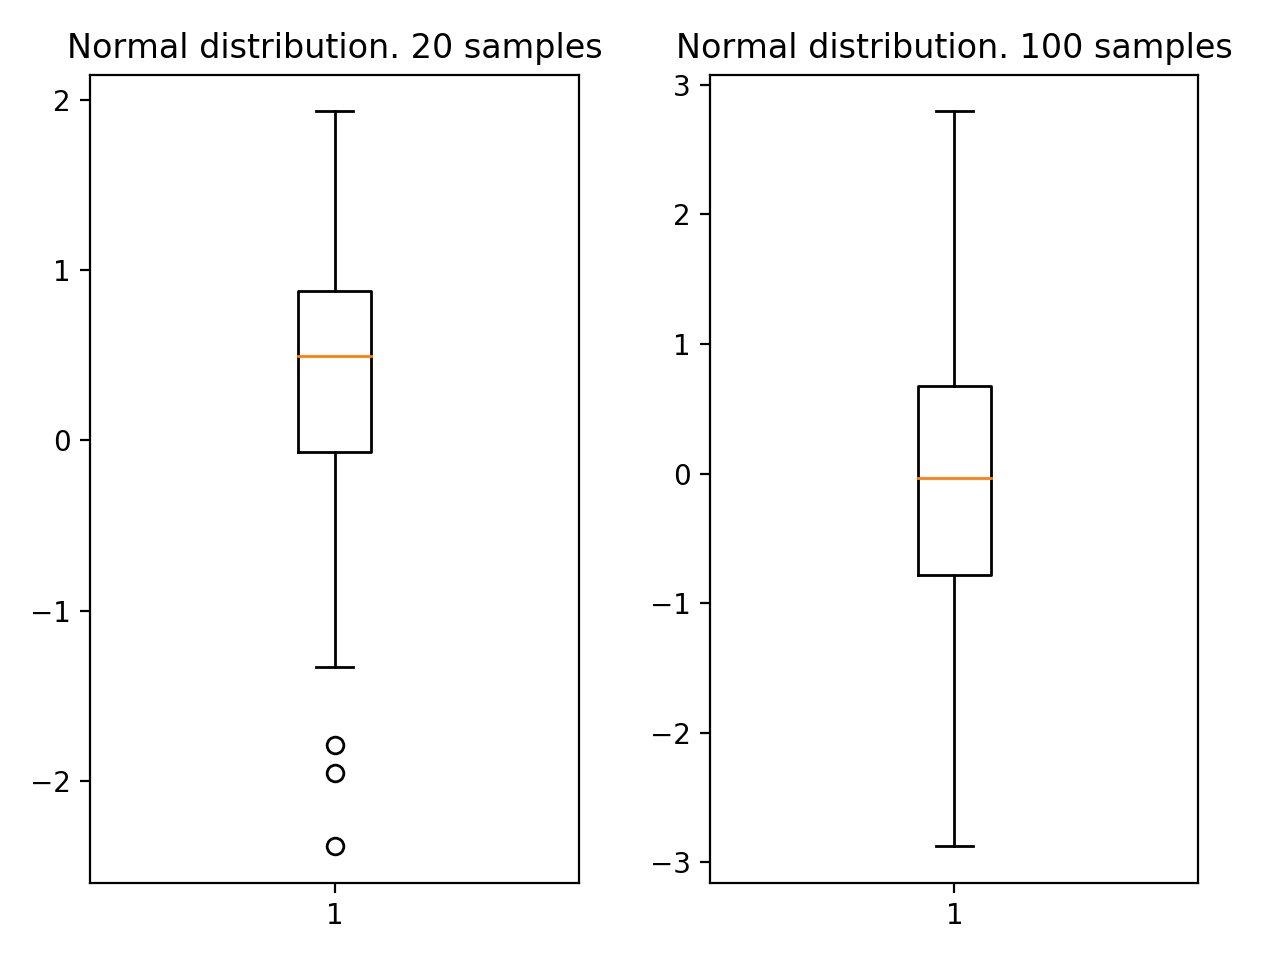
\includegraphics[scale=0.7]{fig/Normal distribution.png}
		\caption{Боксплот Тьюки для нормального распределения} 
		\label{pic:pic_name}
	\end{center}
\end{figure}


\subsection{Распределение Коши}
\begin{figure}[H]
	\begin{center}
		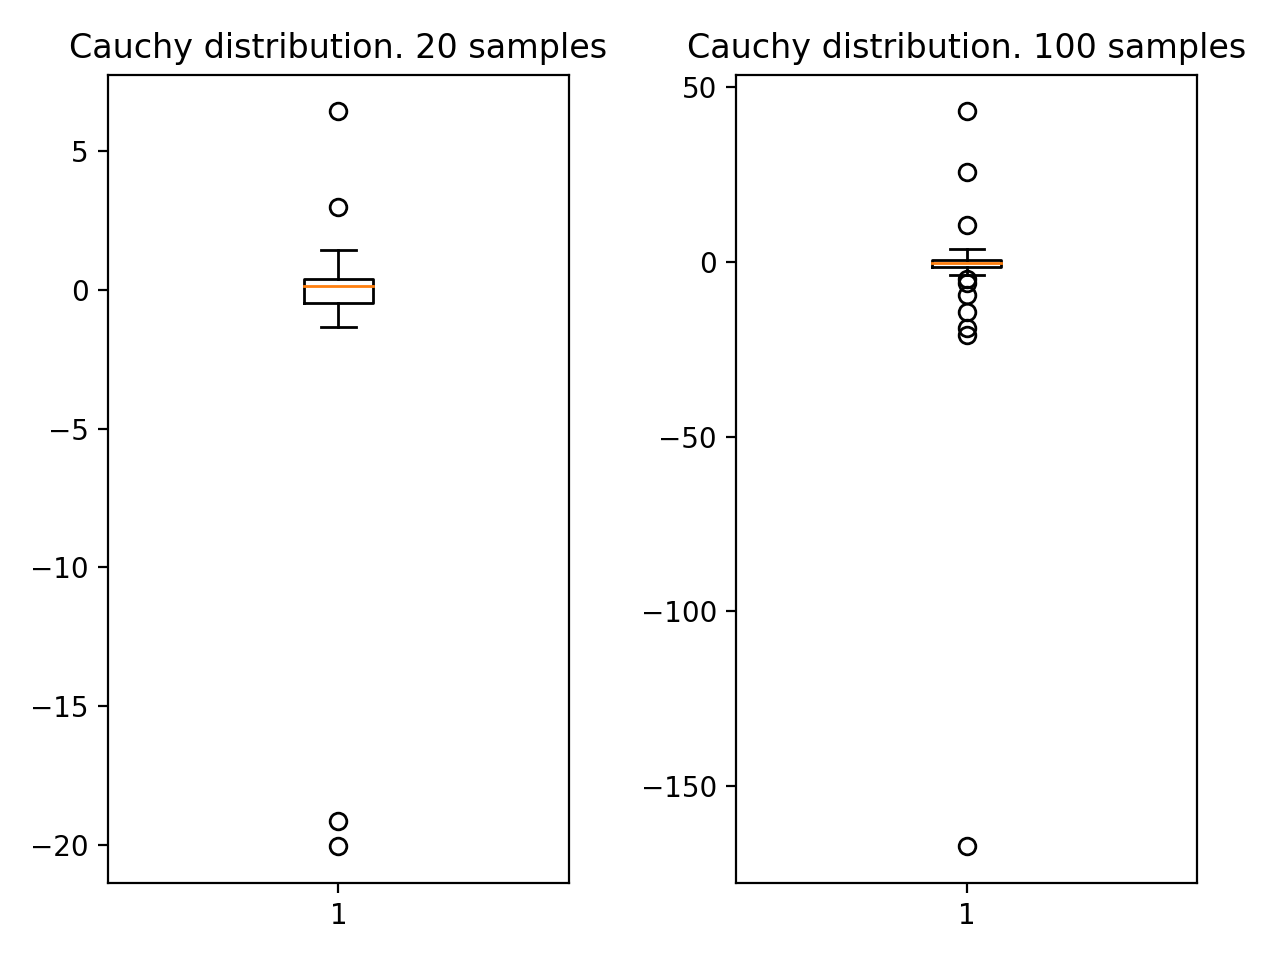
\includegraphics[scale=0.7]{fig/Cauchy distribution.png}
		\caption{Боксплот Тьюки для распределения Коши} 
		\label{pic:pic_name}
	\end{center}
\end{figure}


\subsection{Распределение Лапласа}
\begin{figure}[H]
	\begin{center}
		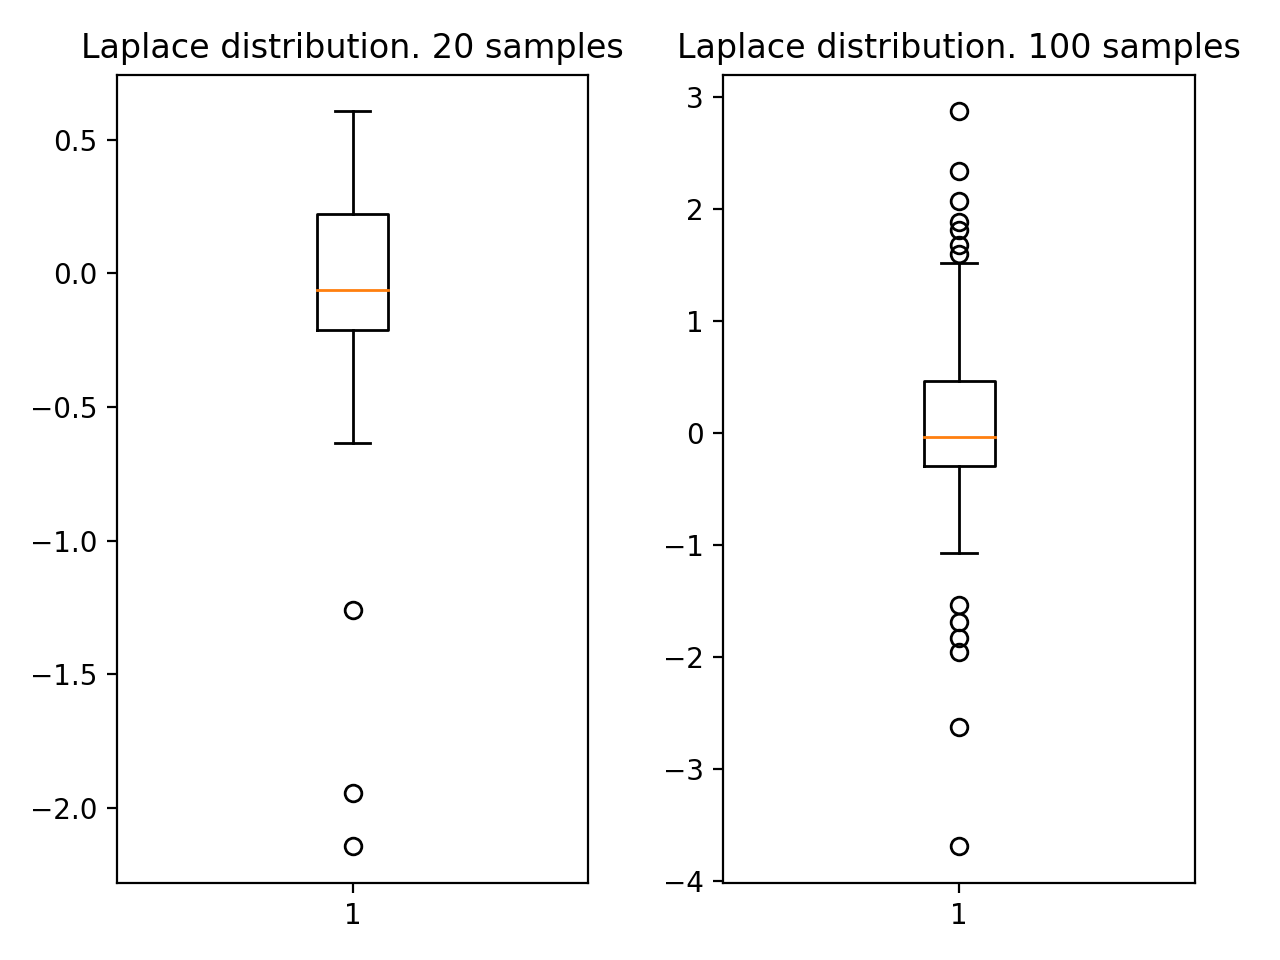
\includegraphics[scale=0.7]{fig/Laplace distribution.png}
		\caption{Боксплот Тьюки для распределения Лапласа} 
		\label{pic:pic_name}
	\end{center}
\end{figure}


\subsection{Распределение Пуассона}
\begin{figure}[H]
	\begin{center}
		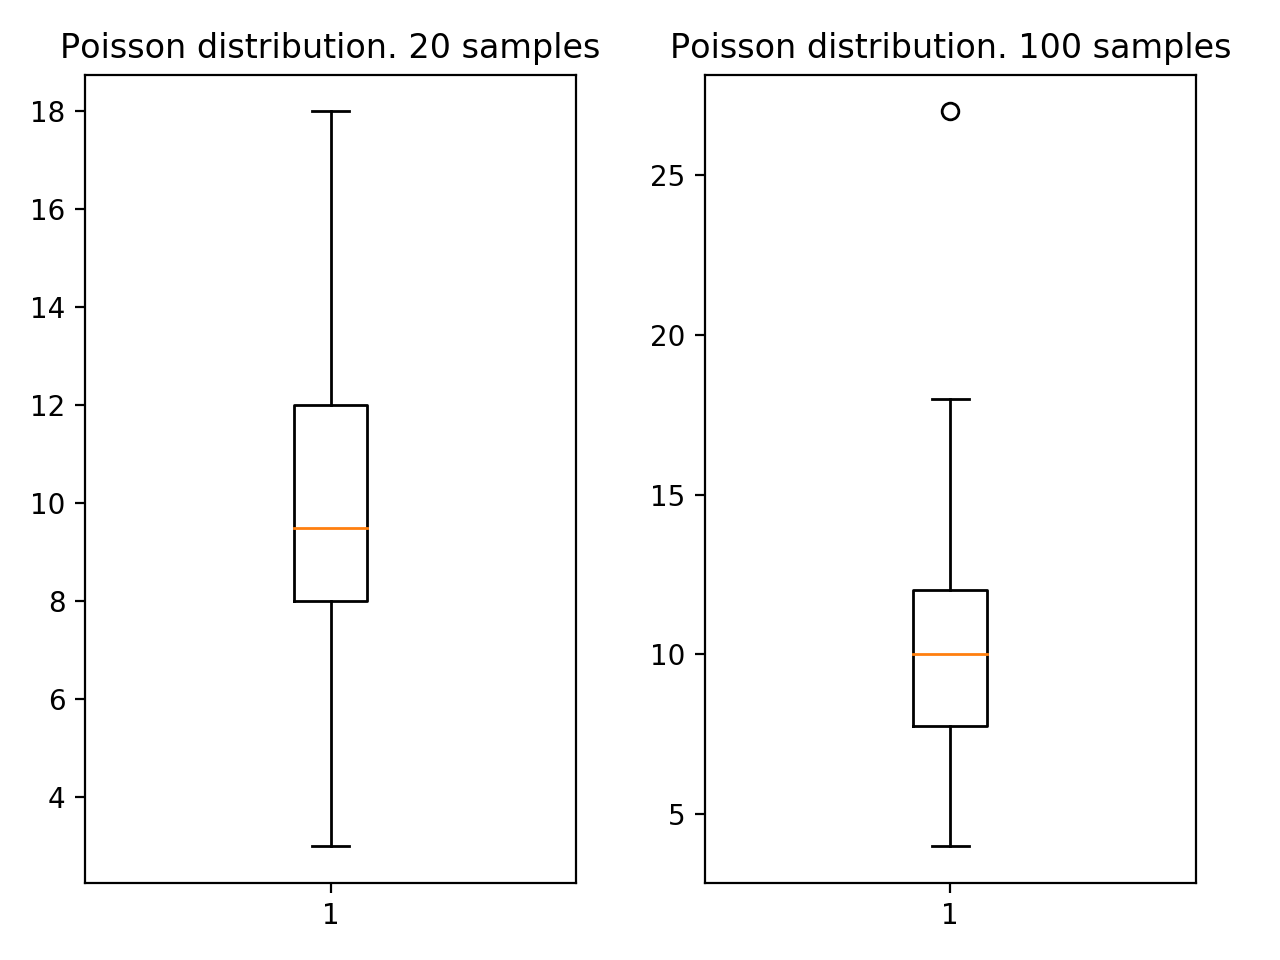
\includegraphics[scale=0.7]{fig/Poisson distribution.png}
		\caption{Боксплот Тьюки для распределения Пуассона} 
		\label{pic:pic_name} 
	\end{center}
\end{figure}


\subsection{Равномерное распределение}
\begin{figure}[H]
	\begin{center}
		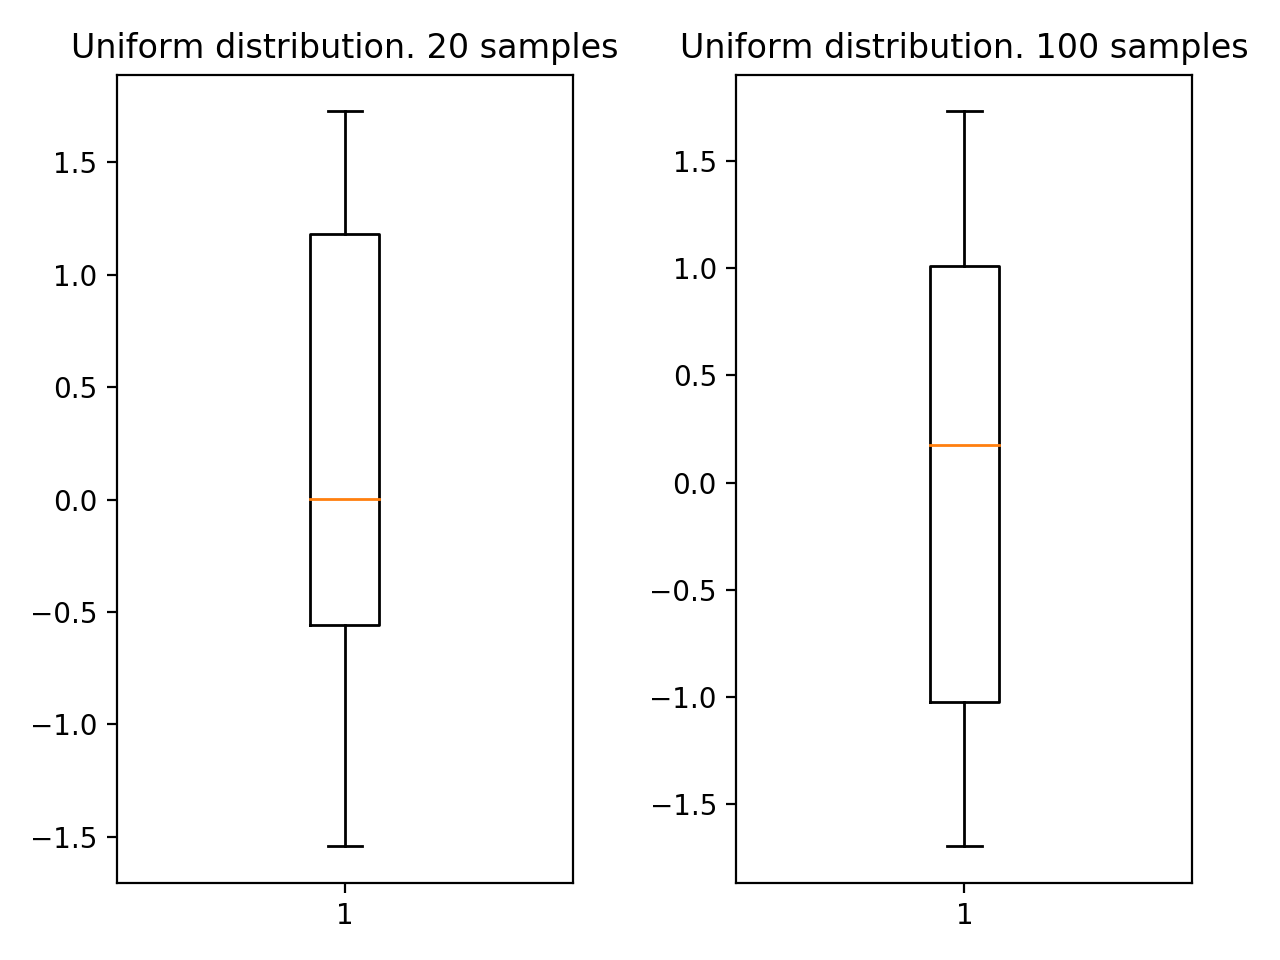
\includegraphics[scale=0.7]{fig/Uniform distribution.png}
		\caption{Боксплот Тьюки данные для равномерного распределения} 
		\label{pic:pic_name}
	\end{center}
\end{figure}



\subsection{Сравнение доли выбросов с теоретической вероятностью}
\begin{table}[H]
\caption{Процент выбросов}
\begin{center}
 \begin{tabular}{||c || c c ||} 
 \hline
 Распределение & n = 20  & n = 100 \\ 
 \hline\hline
  Нормальное  & 0 & 0.01 \\ 
 \hline
 Коши         & 0.05   & 0.12 \\
 \hline
  Лапласа     & 0.05  &  0.04  \\
 \hline
  Пуассона    & 0.05 &  0 \\
 \hline
  Равномерное & 0  &  0  \\
 \hline
\end{tabular}
\end{center}
\end{table}



\begin{table}[H]
\caption{Теоретическая вероятность выбросов}
\begin{center}
 \begin{tabular}{||c || c c c c c||} 
 \hline
 Распределение & \(Q_{1}^T\)  & \(Q_{3}^T\) & \(X_{1}^T\) & \(X_{2}^T\) & \(P_{B}^T\) \\ 
 \hline\hline
  Нормальное  & -0.6745 & 0.6745 & -2.698 & 2.698  & 0.007 \\ 
 \hline
 Коши         & -1      &  1 &  -4 & 4 &  0.156 \\
 \hline
  Лапласа     & -0.490  &  0.490 & -1.961 & 1.961 &  0.063 \\
 \hline
  Пуассона    & 8       &  12 & 2 & 18 &  0.008 \\
 \hline
  Равномерное & -0.866  &  0.866 &  -3.464 & 3.464 & 0.0  \\
 \hline
\end{tabular}
\end{center}
\end{table}



\section{Обсуждение}
Отметим, что наименьший процент выбросов имеют равномерное распределение и распределение Пуассона, затем следует нормальное распределение и распределение Лапласа. Наибольший процент выбросов имеет распределение Коши.


\section{Литература}
Максимов Ю. Д. Математическая статистика //СПб.: СПбГПУ. – 2004.

Гурский Е. И. Теория вероятностей с элементами математической статистики. – Высш. школа, 1971.

\section{Приложения}

Репозиторий с кодом программы и кодом отчёта: \href{https://github.com/unjamini/math-stat-lab}{https://github.com/unjamini/math-stat-lab}





% Не редактируем: Страница библиографии (формируется автоматически из книжек, указанных в refs.bib и пометок \cite{имя_источника} в тексте)
\include{templates/bibpage}
\end{document}
